SQL er nokkuð sveigjanlegt og yfirgripsmikið mál. 
Margt er að læra, í þessum áfanga er einungis farið yfir lítið brot af því sem viðfangsefnið hefur upp á að bjóða.

Byrjum á að skoða grundvallaraðgerðirnar í SQL - það að búa til töflur, setja í þær gögn og að skoða gögnin aftur.
\section{Töflur}
Gögn í SQL-gagnagrunni má líta á sem raðir í töflum. Því hlýtur mikilvægt skref í því að læra að nota SQL að vera það að skilja uppbyggingu taflna mjög nákvæmlega.

Lítum fyrst á dæmigerða töflu.

\begin{table}
\centering
\caption{Nokkrir starfsmenn Tækniskólans}
\label{tafla:starfsmenn_ts}
\begin{tabular}{lll}
\toprule
Nafn&Starfsheiti&Netfang\\
\midrule
Bjargey G. Gísladóttir&Skólastjóri&bbg@tskoli.is\\
Eiríkur Ernir Þorsteinsson&Kennari&eet@tskoli.is\\
Emil Gautur Emilsson&Kennari&ege@tskoli.is\\
% Donatas Butkus&Tölvuþjónusta&db@tskoli.is\\
Geir Sigurðsson&Kennari&ges@tskoli.is\\
Gunnar Þórunnarson&Kennari&gus@tskoli.is\\
Guðmundur Jón Guðjónsson&Kennari&gjg@tskoli.is\\
Guðrún Randalín Lárusdóttir&Kennari&grl@tskoli.is\\
Hallur Ó. Karlsson&Kennari&hal@tskoli.is\\
Konráð Guðmundsson&Kennari&kng@tskoli.is\\
% Matthias Skúlason&Tölvuþjónusta&matti@tskoli.is\\
Sigurður R. Ragnarsson&Kennari&srr@tskoli.is\\
Snorri Emilsson&Kennari&sem@tskoli.is\\
% Tryggvi Jóhannsson&Kerfisstjóri&tj@tskoli.is\\
Þórarinn J. Kristjánsson&Kennari&tjk@tskoli.is\\
\bottomrule
\end{tabular}
\end{table}
Eins og allar alvöru töflur inniheldur þessi starfsmannatafla annarsvegar \emph{dálkheiti} og hins vegar \emph{gögn}. Dálkheitin eru ``Nafn'', ``Starfsheiti'' og ``Netfang''. Dæmi um upplýsingar eru að til sé starfsmaður sem heitir ``Eiríkur Ernir Þorsteinsson'', sem er ``Kennari'' og hefur netfangið ``eet@tskoli.is''. 

Mikilvægt er að átta sig á þessum mun - hver einasta tafla sem unnið er með inniheldur dálkheiti og gögn, sem eru aðskilin fyrirbrigði. Þetta á augljóslega við ``hefðbundnar'' töflur sem við sjáum á prenti og í forritum á borð við Microsoft Excel. En taktu eftir því að þetta á en líka við töflur sem við skilgreinum með SQL-skipunum.

Þegar töflur eru sýndar á prenti er venjan að dálkheitin komi fram í fyrstu línu töflunnar (og oftast aðskilin gögnunum með striki). Gögnin koma fram í næstu línum.

Þegar SQL er notað til að lýsa töflum eru dálkheitin og aðrar upplýsingar sem skilgreina töfluna sjálfa búnar til með sérstökum skipunum. Aðrar skipanir eru notaðar til að vinna með gögnin sjálf. Við sjáum dæmi um þessar skipanir í undirkaflanum \nameref{undirkafli:synidaemi_i_sql}. 6\footnote{Betur verður farið í muninn á þessum skipunum í kafla \ref{kafli:uppfaera}}
\section{Fyrirspurnir}
Ekki er mikið gagn í því að geyma upplýsingar í töfluformi nema að hægt sé að ná í þær aftur.

Einfalt er að fletta upp upplýsingum í litlum töflum á borð við töflu \ref{tafla:starfsmenn_ts}. Viljum við t.d. komast að því hver er með netfangið ``kng@tskoli.is'' dugar okkur að láta augun reika yfir töfluna þar til við rekumst á netfangið og líta svo í starfsmannadálkinn.

Væri taflan örlítið stærri væri verkefnið strax erfiðara. Væri taflan á stærð við símaskrána væri það nær ómögulegt.

Slíkar uppflettingar, stórar og smáar, eru sérsvið SQL. Þær eru nefndar \emph{fyrirspurnir} og eru framkvæmdar með mjög mikilvægri SQL-skipun sem heitir \emph{SELECT}. Við sjáum dæmi um SELECT-skipanir í undirkaflanum \nameref{undirkafli:synidaemi_i_sql} og kynnumst þeim náið í kafla \ref{kafli:select}.
\section{Gagnagrunnar}
Ef upplýsingar eru geymdar í töflum, hvað er þá gagnagrunnur?

Gagnagrunnur heldur utan um töflur, eina eða fleiri. Hann bindur þær saman í eina heild og myndar um þær umgjörð.
\begin{marginfigure}
\centering
\caption{Uppbygging gagnagrunns}
\label{mynd:uppbygging}
\color{red} Hingað kemur falleg mynd af uppbyggingu gagnagrunna.
\end{marginfigure}

\section{Sýnidæmi í SQL}
\label{undirkafli:synidaemi_i_sql}
Skoðum hvernig búa má til töflu \ref{tafla:starfsmenn_ts} með SQL, setja í hana gögn og sækja gögnin aftur. 

Eins og fram hefur komið þarf til þess að nota SQL-skipanir.

\begin{example}[h]
\caption{CREATE skipun fyrir starfsmannatöfluna}
\label{sql:k2d1}
\centering
\sql{sql/k2d1.sql}
\end{example}

Skipunina til að skilgreina töfluna má sjá á SQL-sýnidæmi \ref{sql:k2d1}. Þetta er mjög dæmigerð skipun til að búa til töflu. Þar kemur fram hvað gera skal (búa til töflu $\rightarrow$ \verb|CREATE TABLE|) og hver dálkheitin eru (nafn, Starfsheiti og netfang). Í kafla \ref{kafli:uppsetningtaflna} skoðum við hin orðin sem koma fyrir í skipuninni og í kafla \ref{undirkafli:keyrslaiworkbench} sjáum við hvernig koma má skipuninni í gagnið.

Hér ber að athuga að enn eru engin gögn komin inn í töfluna. Það má gera með skipuninni í SQL-sýnidæmi \ref{sql:k2d2}.

\begin{example}[h]
\caption{INSERT skipun fyrir starfsmannatöfluna}
\label{sql:k2d2}
\centering
{\small
\sql{sql/k2d2.sql}
}
\end{example}

Til að sækja gögn úr töflunni þarf síðan að framkvæma fyrirspurn. Dæmi um fyrirspurn (SQL-skipun) sem finnur nafn þess starfsmanns sem er með netfangið ``kng@tskoli.is'' má sjá á sýnidæmi \ref{sql:k2d3}.

\begin{example}[h]
\caption{SELECT skipun sem finnur Konráð kennara í starfsmannatöflunni}
\label{sql:k2d3}
\centering
\sql{sql/k2d3.sql}
\end{example}

\section{Keyrsla í MySQL Workbench}
\label{undirkafli:keyrslaiworkbench}
Lítum örstutt á hvernig nota má MySQL Workbench til að búa til okkar fyrstu töflu með SQL.

Um nokkur skref er að ræða.
\begin{enumerate}
 \item Ræsa þarf forritið. Við það birtist upphafsskjár, líkur þeim sem sjá má á mynd \ref{mynd:workbench-upphafsskjar}.\footnote{Útlit MySQL Workbench er eðli málsins samkvæmt örlítið mismunandi eftir stýrikerfum og útgáfum á forritinu. Skjáskotin eru tekin af Workbench útgáfu 6.0, á Linux vél.}
 \item Mynda þarf tengingu við MySQL-server. Henni þarf að gefa nafn, IP-tölu MySQL serversins, notandanafn og lykilorð.\footnote{Nemendur Tölvudeildar Tækniskólans skulu biðja kennarann um þessar upplýsingar.} Sjá mynd \ref{mynd:workbench-login}.
 \item Búa þarf til nýjan gagnagrunn á MySQL-servernum á skjánum sem birtist eftir að tengingin er mynduð. Það er einfaldast að gera með svokallaðri \verb|CREATE DATABASE| skipun, slegin inn í aðalgluggann - sjá mynd \ref{mynd:workbench-create-db}. Þegar þessu er lokið höfum við keyrt okkar fyrstu SQL-skipun!
 \item Skipunin í sýnidæmi \ref{sql:k2d1} er slegin inn í aðalgluggann og keyrð. Taflan er þá komin inn!
\end{enumerate}
Ávallt má gera ráð fyrir að SQL-sýnidæmi í þessari bók megi keyra með hliðstæðum hætti - í aðalglugga MySQL Workbench. T.d. mætti keyra sýnidæmi \ref{sql:k2d2} og \ref{sql:k2d3} á þann hátt.

\begin{figure*}
\caption[Upphafsskjár MySQL Workbench]{Upphafsskjár MySQL Workbench. Örin vísar á hnapp sem nota má til að búa til nýja tengingu.}
\label{mynd:workbench-upphafsskjar}
\centering
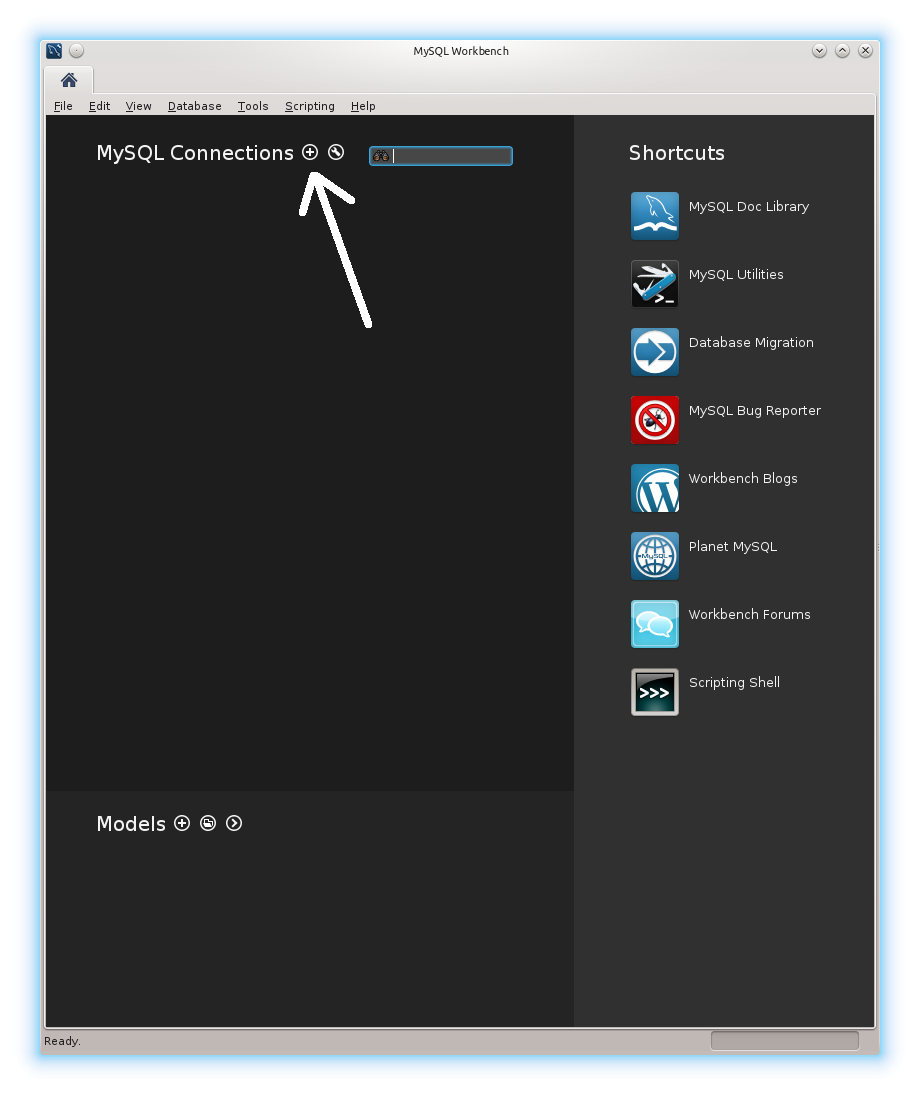
\includegraphics[width=\linewidth]{myndir/workbench-upphafsskjar-or}
\end{figure*}

\begin{figure*}
\caption[Tengingarskjár MySQL Workbench]{Tengingarskjár MySQL Workbench. Hér er verið að búa til tenginguna ``Prufutenging'', sem tengist MySQL-þjóni sem keyrir á sömu tölvu og Workbench-inn (127.0.0.1) með notandanafninu ``root''.}
\label{mynd:workbench-login}
\centering
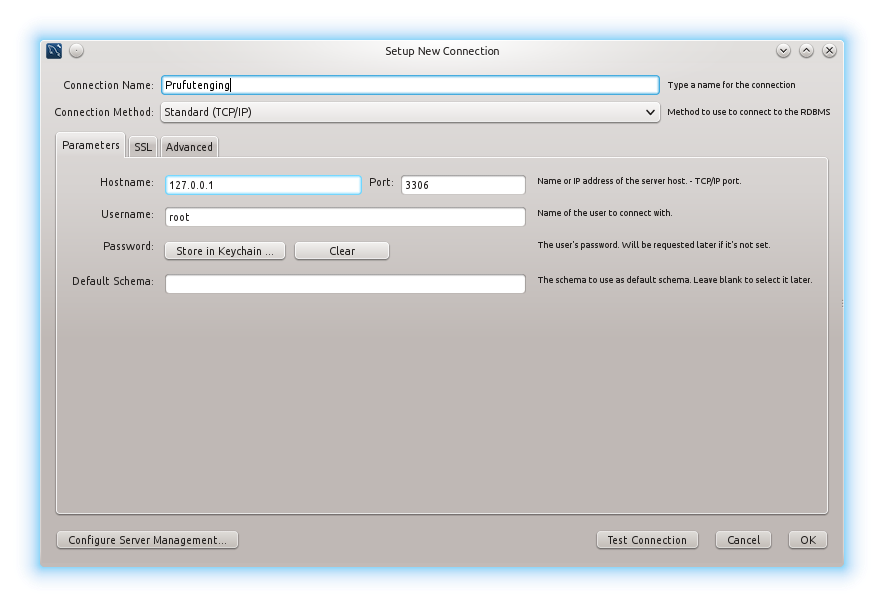
\includegraphics[width=\linewidth]{myndir/workbench-login}
\end{figure*}

\begin{figure*}
\caption[Nýr gagnagrunnur]{Nýr gagnagrunnur búinn til með MySQL Workbench. Efri örin vísar á hnappinn sem ýta þarf á til að keyra SQL-skipunina. Neðri örin vísar á lista af gagnagrunnum sem sýnilegir eru á servernum. Birtist gagnagrunnurinn sem búinn er til ekki um leið og skipunin er keyrð, hægri-smellið þá á listann og ``refresh''ið hann.}
\label{mynd:workbench-create-db}
\centering
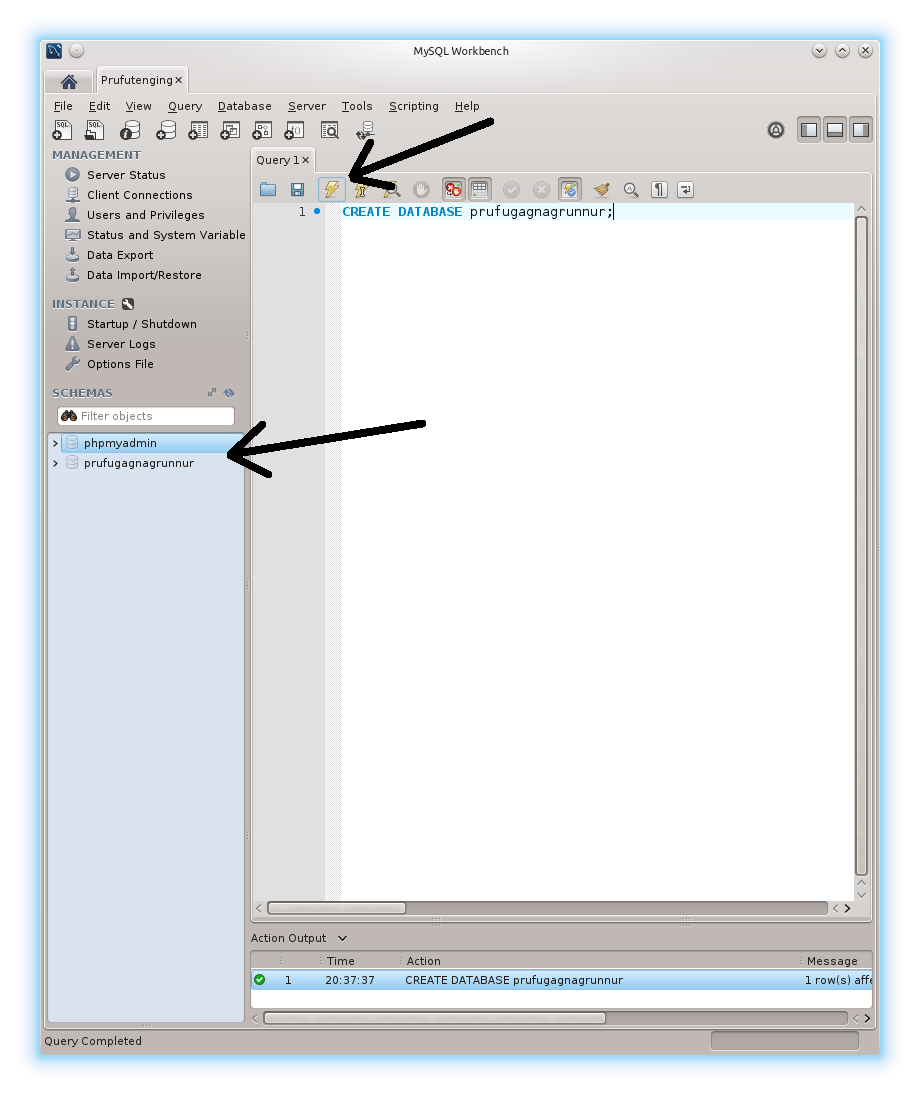
\includegraphics[width=0.8\linewidth]{myndir/workbench-create-db-or}
\end{figure*}

\begin{figure*}
\caption[Ný tafla]{Ný tafla búin til með MySQL Workbench. Skipunin er slegin inn í aðalgluggann og keyrð með ``eldingarhnappnum'' eins og skipunin á mynd \ref{mynd:workbench-create-db}.}
\label{mynd:workbench-create-table}
\centering
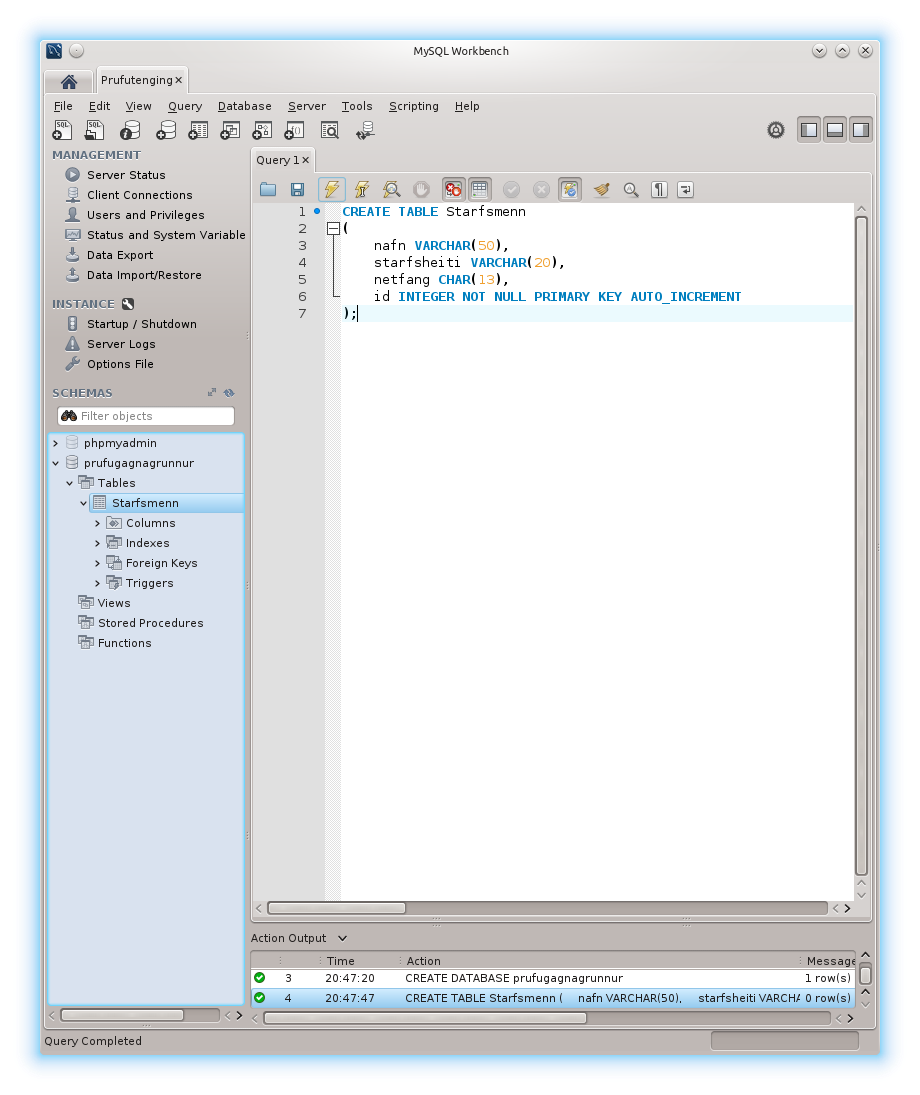
\includegraphics[width=0.8\linewidth]{myndir/workbench-create-table}
\end{figure*}

\section{Yfirlit}
Í þessum kafla fengum við örstutta kynningu því hvernig SQL-gagnagrunnar eru uppbyggðir og hvernig við getum átt við þá samskipti. 

Helstu atriðin eru:
\begin{itemize}
 \item Gögn í SQL-gagnagrunni má líta á sem raðir í töflum.
 \item SQL-skipanir eru notaðir til að skilgreina töflur og setja í þær gögn.
 \item Fyrirspurnir eru notaðar til að sækja gögn úr gagnagrunnum. Fyrirspurnir eru sérstök gerð SQL-skipana.
 \item SQL-skipanir má keyra úr aðalglugga MySQL Workbench.
\end{itemize}
Athuga ber að við höfum ekki farið yfir uppbyggingu skipananna. Það að læra á skipanirnar sjálfar er viðfangsefni næstu kafla.